\documentclass[tikz, border=2mm]{standalone}

\usepackage{tikz}
\usetikzlibrary{positioning, calc, backgrounds, shapes.geometric}
\usepackage{amsmath}

% --- CUSTOM COLORS ---
\definecolor{deepred}{HTML}{73000A}

\begin{document}

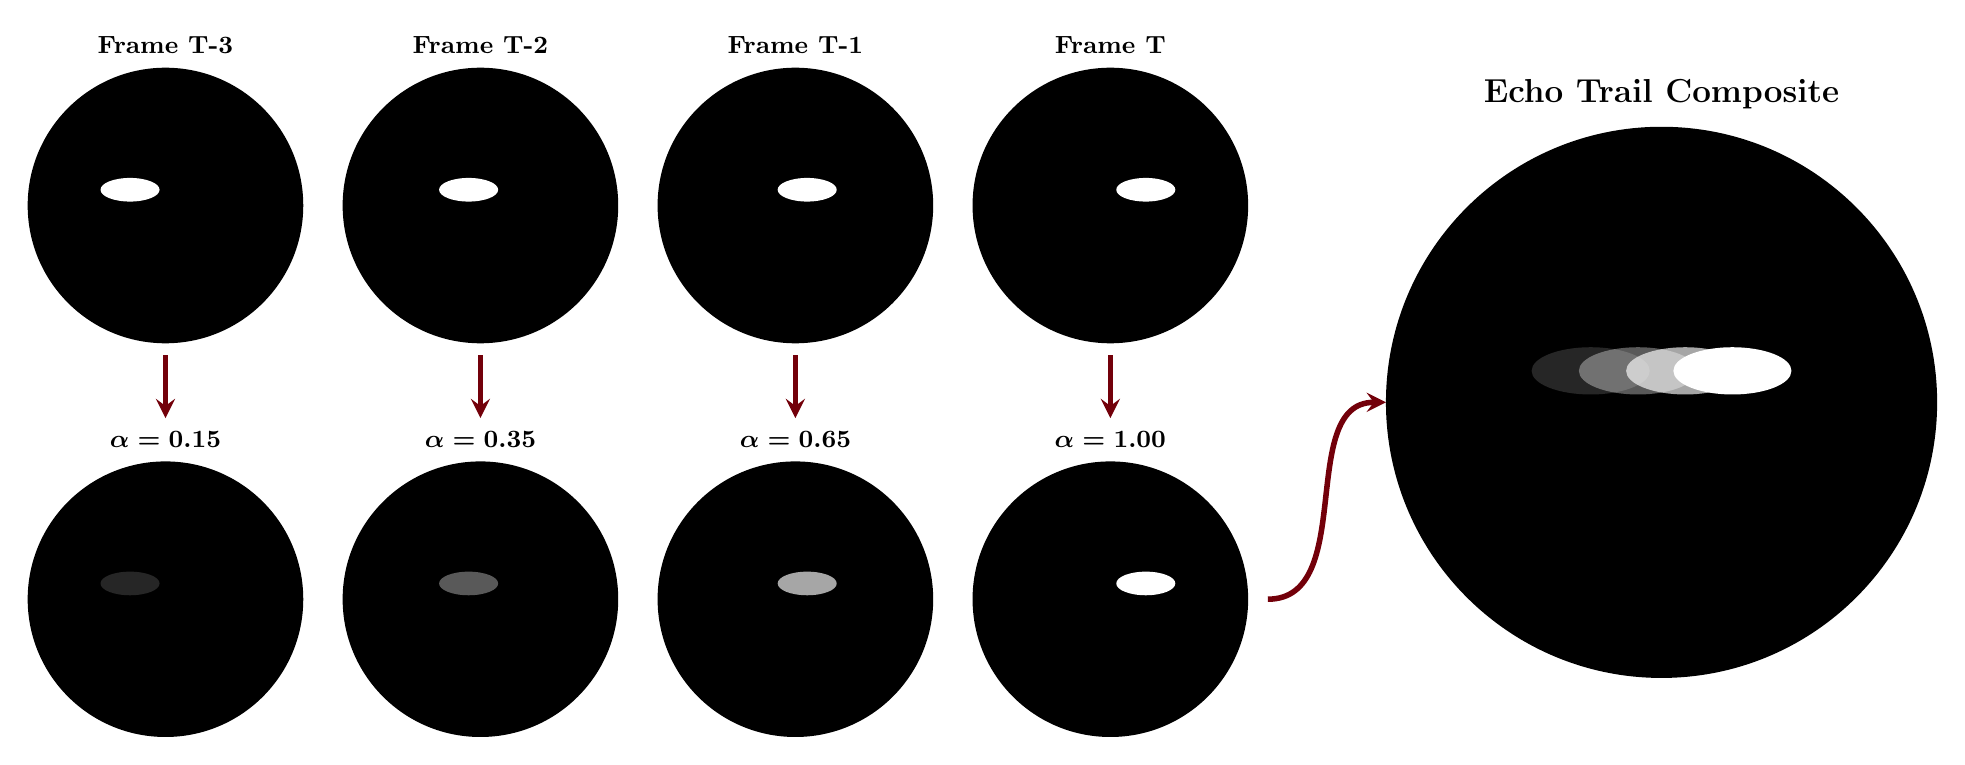
\begin{tikzpicture}[
    target/.style={
        ellipse,
        fill=white,
        minimum width=0.75cm,
        minimum height=0.3cm,
        inner sep=0pt
    }
]

% --- RANDOM SEED ---
\pgfmathsetseed{100}

% --- MACRO: DRAW FRAME ---
\newcommand{\drawframe}[4]{
    \begin{scope}[shift={#4}]
        \fill[black] (0,0) circle (1.75cm);
        \begin{scope}
            \clip (0,0) circle (1.75cm);
            \node[target, opacity=#3] at (#2, 0.2) {};
        \end{scope}
        \node[above, align=center, font=\bfseries\small] at (0, 1.8) {#1};
    \end{scope}
}

% --- MACRO: DRAW BIG COMPOSITE ---
\newcommand{\drawbigcomposite}[1]{
    \begin{scope}[shift={#1}]
        \fill[black] (0,0) circle (3.5cm);
        \begin{scope}
            \clip (0,0) circle (3.5cm);
            \tikzset{
                bigtarget/.style={
                    ellipse,
                    fill=white,
                    minimum width=1.5cm,
                    minimum height=0.6cm,
                    inner sep=0pt
                }
            }
            \node[bigtarget, opacity=0.15] at (-0.9, 0.4) {};
            \node[bigtarget, opacity=0.35] at (-0.3, 0.4) {};
            \node[bigtarget, opacity=0.65] at (0.3, 0.4) {};
            \node[bigtarget, opacity=1.0]  at (0.9, 0.4) {};
        \end{scope}
        \node[above, align=center, font=\bfseries\large] at (0, 3.6)
            {Echo Trail Composite};
    \end{scope}
}

% --- ROW 1 ---
\drawframe{Frame T-3}{-0.45}{1.0}{(0,0)}
\drawframe{Frame T-2}{-0.15}{1.0}{(4,0)}
\drawframe{Frame T-1}{0.15}{1.0}{(8,0)}
\drawframe{Frame T}{0.45}{1.0}{(12,0)}

% --- ROW 2 ---
\drawframe{$\boldsymbol{\alpha=0.15}$}{-0.45}{0.15}{(0,-5)}
\drawframe{$\boldsymbol{\alpha=0.35}$}{-0.15}{0.35}{(4,-5)}
\drawframe{$\boldsymbol{\alpha=0.65}$}{0.15}{0.65}{(8,-5)}
\drawframe{$\boldsymbol{\alpha=1.00}$}{0.45}{1.0}{(12,-5)}

% --- COMPOSITE ---
\drawbigcomposite{(19,-2.5)}

% --- ARROWS ---
\begin{scope}[deepred, line width=2pt, >=stealth]
    \draw[->] (0, -1.9) -- (0, -2.7);
    \draw[->] (4, -1.9) -- (4, -2.7);
    \draw[->] (8, -1.9) -- (8, -2.7);
    \draw[->] (12, -1.9) -- (12, -2.7);
    \draw[->] (14, -5) to[out=0, in=180] (15.5, -2.5);
\end{scope}

\end{tikzpicture}

\end{document}
